\chapter{5}
\label{chapter:incremental}

\section{ステッパの動作}

本章で説明する incremental なステッパは、表面上は \ref{chapter:try-with} 章のステッパと同じ動作をするが、
内部での処理方法および速さが大きく異なる。
本節では、既存のステッパと本章の incremental なステッパのそれぞれの動作について説明する。

いずれのステッパも、実行可能な1つのプログラムを対象としている。

\subsection{DrRacketのステッパ}
\label{ステッパの動作-DrRacketのステッパ}
DrRacket のステッパ\cite{clements01}は、ユーザが入力したプログラムを全ステップの情報を生成するプログラムへ変換し、それを実行してステップの情報を蓄えながら、ユーザの操作に従って1つのステップを表示する。実行開始に少し遅れて、表示のための処理を並列して行うことになる。

\subsection{incremental でない OCaml ステッパ}
\label{ステッパの動作-incrementalでないOCamlステッパ}

\ref{chapter:try-with} 章で実装した OCaml ステッパ (以下、incremental でない OCaml ステッパ) では、
では、インタプリタにステップ出力機能を足したものに入力プログラムを渡し、
全ステップの文字列を生成する。
プログラムを全て実行するかステップ数の上限に達すると実行を終了し、
最初のステップを表示し、
ユーザの操作に従って表示するステップを変える。

インタプリタは新しく我々が作った OCaml の関数であり、通常のインタプリタよりも実行速度が遅い。そこにさらに出力機能を足したインタプリタによるプログラム実行が終わるまで表示が始まらないため、実行に時間がかかるプログラムのステップ実行をするには長い時間待つ必要がある。

\subsection{提案するステッパ}
\label{ステッパの動作-提案するステッパ}

本章で提案するステッパは、インタプリタにステップ出力機能を足したものに入力プログラムを渡し、1ステップの簡約を計算したらただちにそのステップを出力し、続きの実行は行わずにプロセスを終了する。ユーザから次のステップを表示するなどの命令がされ次第、前回の出力の一部を新しい入力として受け取って次の1ステップ実行をする。

例えば、\texttt{2 * 3 + 5 * 7} というプログラムを入力されると、incremental でないステッパは \texttt{2 * 3 + 5 * 7 $\leadsto$ 2 * 3 + 35 $\leadsto$ 6 + 35 $\leadsto$ 41} という3ステップを出力するのに対して、incremental なステッパは \texttt{2 * 3 + 5 * 7 $\leadsto$ 2 * 3 + 35} の1ステップを出力する。次のステップを表示する命令がされたときに、外部のプログラムがそこから \texttt{2 * 3 + 35} という部分を抜き出して再度ステッパに入力することでその次のステップを得る。

incremental なステッパには、メモリに膨大なステップの情報を保存する必要がない、ユーザが見ないステップは計算されないという特徴がある。



\section{OCaml の attribute}
\label{OCamlのattribute}
OCaml 4.02 以降では、OCaml の構文木中に attribute
という情報を付加することができる。
attribute はそれぞれ名前と、
OCaml のプログラムやシグネチャなどの引数を持つ。
incremental でない OCaml ステッパ (\ref{section:ocaml stepper} 節) および
本章で提案するステッパでは attribute を利用している。
本節では、本章のステッパの実装で利用する種類の attribute を紹介する。

\subsection{式の attribute}
\label{OCamlのattribute-式のattribute}

\begin{figure}
  \begin{center}
    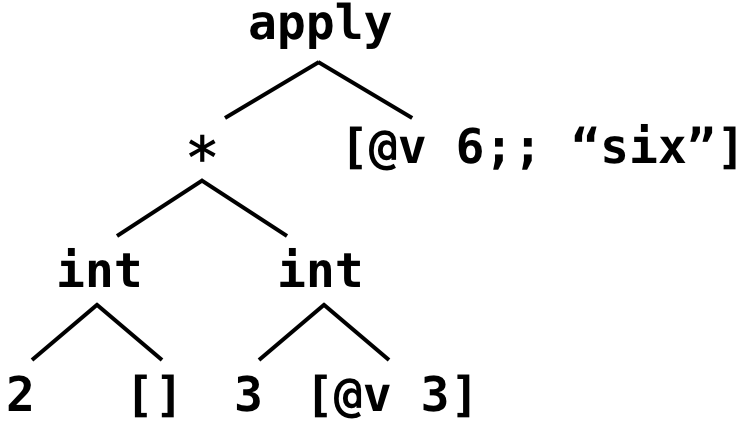
\includegraphics[width=5.2cm, height=3cm]{5/attribute.png}
  \end{center}
  \caption{attribute を含む構文木の例}
  \label{figure:attribute}
\end{figure}

OCaml のプログラムでは、任意の部分式に attribute をつけることができる。
式 \texttt{e} に OCaml プログラム \texttt{P} を引数に持つ
\texttt{name} という attribute を付けたものは \texttt{e[@name P ]} と書く。
例えば \texttt{(2 * 3[@v 3])[@v 6;; "six" ]} という式は大まかには図
\ref{figure:attribute} のように構文解析され、
ステッパプログラムのように構文木を扱うプログラムの中で
attribute の内容を利用することができる。
通常の OCaml コンパイラは attribute を無視するので、
シンタックスエラー等を起こしてしまう場合を除いて、
attribute が付いた式と付いていない式で意味は変わらない。

\begin{figure}
\begin{alltt}
  (* Step 0 *)                              (* Step 0 *)
  (2 * 3) + (5 * 7)[@stepper.redex ]        (2 * 3) + \colorbox{lightgreen}{(5 * 7)}
  (* Step 1 *)                              (* Step 1 *)
  (2 * 3) + 35[@stepper.reduct ]            (2 * 3) + \colorbox{purple}{35}
  (* Step 1 *)                              (* Step 1 *)
  (2 * 3)[@stepper.redex ] + 35             \colorbox{lightgreen}{(2 * 3)} + 35
  (* Step 2 *)                              (* Step 2 *)
  6[@stepper.reduct ] + 35                  \colorbox{purple}{6} + 35
  (* Step 2 *)                              (* Step 2 *)
  (6 + 35)[@stepper.redex ]                 \colorbox{lightgreen}{(6 + 35)}
  (* Step 3 *)                              (* Step 3 *)
  41[@stepper.reduct ]                      \colorbox{purple}{41}
\end{alltt}
\caption{ハイライトのための attribute の利用}
\label{figure:highlight}
\end{figure}

incremental でない OCaml ステッパでは、
各ステップで簡約が起こっている部分の式をハイライトして示すために
attribute を利用している。
例えば \texttt{(2 * 3) + (5 * 7)} というプログラムに対する
incremental でないステッパの出力は図 \ref{figure:highlight} の左の文字列である。
インタフェースを受け持つプログラムはこの文字列を受け取り、
図\ref{figure:highlight}の右側のように、
attribute が付いた式をハイライトし、
さらに attribute を表す文字列を削除した上で表示している。

本章の incremental なステッパでも、
同様の方法で簡約部分のハイライトを行う。
本論文では、ステッパの出力文字列中のハイライトのための attribute を省略したり、
緑色および紫色のハイライトで現すことがある。

\subsection{プログラムの attribute}
\label{OCamlのattribute-プログラムのattribute}
attribute はプログラム自体にも付けることができる。

OCaml のプログラムは structure item の列であり、
structure item には式、変数定義(\texttt{let 変数名 = 式})、
型定義、モジュール定義、attribute などの種類がある。
structure item の間には \texttt{;;} を書くことで明示的に structure item の境を示すことができる。

attribute の structure item はプログラム中に何度でも書くことができ、
名前の重複などに関する制約も無い。
また式に付ける attribute と同じく、
標準のコンパイラなどはこれを無視するのでプログラムの意味に影響を与えない。

\texttt{name} という名前で OCaml プログラム\texttt{P}
を含む attribute の structure item を \texttt{[@@@name P ]} と書く。
例えば \texttt{let a = 1 [@@@name1 1;; 2 + 3 ] let b = 2 [@@@name2 ]}
というプログラムは、
(1)\texttt{a} の定義、(2)\texttt{1} と \texttt{2 + 3}
を引数に持つ \texttt{name1} という attribute、(3)\texttt{b} の定義、
(4)引数なしの \texttt{name2} という attribute、
の4つの structure item のリストとして処理され、
それぞれの attribute の内容はステッパが参照することができる。

これを用いると、プログラムに自由に情報を付加することができる。
incremental なステッパの実装において、
副作用によって変化する「状態」や現在のステップ番号を記録するために使用している。


\section{生じる問題と解決方法}
\label{生じる問題と解決方法}

incremental でない OCaml ステッパと全く同じようにステップ出力を行うと、
incremental なステッパでは様々な問題が起きた。
本節ではその問題と、回避するために行った出力内容の変更について説明する。

\subsection{情報の消失}
\label{生じる問題と解決方法-情報の消失}

\subsubsection{問題点}
\label{生じる問題と解決方法-情報の消失-問題点}
\ref{ステッパの動作-DrRacketのステッパ} 節および \ref{ステッパの動作-incrementalでないOCamlステッパ} 節で紹介した既存のステッパは、ステップ実行をした結果を蓄えておき、ユーザが表示ステップを切り替える際にその中から表示するステップの情報を検索して表示するので、ステップ番号を指定すれば任意のステップをすぐに表示することができる。それに対して本研究で提案するステッパは、表示を切り替える命令が入力されるたびに1ステップ先や1ステップ前を計算することになる。その際のステッパの入力は前回出力したプログラムの一部である。すると、1ステップ前を計算する時に問題が起きる。

例えば、\texttt{2 * 3 + 5 * 7} というプログラムをステップ実行するとき、最初に表示される1ステップ目は\texttt{2 * 3 + 5 * 7 $\leadsto$ 2 * 3 + 35}であり、次ステップ表示命令が入力されると今度は \texttt{2 * 3 + 35} を入力として \texttt{2 * 3 + 35 $\leadsto$ 6 + 35} を出力する。ここで前ステップ表示命令が入力された時に、 \texttt{2 * 3 + 35} や \texttt{6 + 35} という情報から \texttt{2 * 3 + 5 * 7 $\leadsto$ 2 * 3 + 35} を導き出すことは不可能である。これは計算が不可逆的であるという性質によるものである。すなわち式 \texttt{5 * 7} と \texttt{35} のどちらからもその値が \texttt{35} だという情報は得られるが、式 \texttt{35} からそれがかつて \texttt{5 * 7} だったという情報は得られないのである。

\subsubsection{解決方法}
\label{生じる問題と解決方法-情報の消失-解決方法}

incremental なステッパでは、簡約後の式に簡約前の式の情報を、簡約された式を表す attribute \texttt{[@stepper.reduct ]} の引数として付加することで、簡約によって失われた情報を復元可能にする。「\texttt{式2} が簡約された結果の \texttt{式1}」を \texttt{式1[@stepper.reduct 式2]} と表して、\texttt{2 * 3 + 5 * 7 $\leadsto$ 2 * 3 + 35} の代わりに \texttt{2 * 3 + 5 * 7 $\leadsto$ 2 * 3 + 35[@stepper.reduct 5 * 7 ]}、また \texttt{2 * 3 + 35 $\leadsto$ 6 + 35} の代わりに \texttt{2 * 3 + 35[@stepper.reduct 5 * 7 ] $\leadsto$ 6[@stepper.reduct 2 * 3 ] + 35[@stepper.reduct 5 * 7 ]} を出力すると、どのステップの出力からでもオリジナルのプログラムまで情報を復元することができる。

さらに、直前のステップで簡約された式が明示的に分かるように、簡約された時のステップ番号も attribute に含める。例えば \texttt{6[@stepper.reduct 2 * 3 ] + 35[@stepper.reduct 5 * 7 ]} に \texttt{2 * 3} や \texttt{5 * 7} のそれぞれの簡約が行われた当時のステップ番号を追加して、\texttt{6[@stepper.reduct (2, 2 * 3) ] + 35[@stepper.reduct (1, 5 * 7) ]} と出力する。こうすると、ここから前のステップを求めるときに、最後に簡約されたのは \texttt{6} だとステップ番号から分かり、\texttt{6} をその attribute に記録された簡約前の式 \texttt{2 * 3} に置き換えることで前のステップ \texttt{2 * 3 + 35[@stepper.reduct (1, 5 * 7) ] $\leadsto$ 6[@stepper.reduct (2, 2 * 3) ] + 35[@stepper.reduct (1, 5 * 7) ]} が得られる。

\subsection{表示の崩れ}
\label{生じる問題と解決方法-表示の崩れ}
\subsubsection{問題点}
OCaml プログラムは、ライブラリで用意された関数を使うと文字列として出力することができ、本研究のステッパではその関数を利用する。その関数は、適当に改行やインデントを入れてプログラムを出力する。しかし、図\ref{figure:highlight} のように attribute が付いたプログラムを出力させて後から外部で attribute を消すと、プログラムの体裁が崩れてしまう可能性がある。

特に、\ref{生じる問題と解決方法-情報の消失-解決方法}節で示したように、簡約後の式に簡約前の式の情報を含む attribute を付けるようにしてステップ実行を進めると、attribute 付きの式の出力が複数行にわたってしまうことがある。すると、例えば
\begin{verbatim}
((2 * 3)
  [@reduct 長い式 ]) +
  (5 * 7)
\end{verbatim}
といった式の途中に改行が入った状態になり、外部のインタフェース用プログラムがこの文字列を受け取って
\begin{verbatim}
(2 * 3) + (5 * 7)
\end{verbatim}
と改行やスペースを調整して表示するのは難しい。

\subsubsection{解決方法}
\label{生じた問題と解決方法-表示の崩れ-解決方法}
我々は、実行に必要な情報がすべて含まれた式「処理用の式」と、表示するための整った式「表示用の式」をそれぞれ出力することでこれを解決した。

具体的には、\texttt{2 * 3 + 5 * 7} の最後のステップの出力が以下のようになるようにした。
\begin{verbatim}
  (* Step 2 *)
  [@@@stepper.process
    6[@stepper.reduct (2, 2 * 3) ] + 35[@stepper.reduct (1, 5 * 7) ] ]
  (6 + 35)[@x ]

  (* Step 3 *)
  [@@@stepper.process 41[@stepper.reduct (3,
    6[@stepper.reduct (2, 2 * 3) ] + 35[@stepper.reduct (1, 5 * 7) ] )] ]
  41[@t ]
\end{verbatim}
すなわち、
\begin{enumerate}
\item 処理用の簡約前の式(\texttt{[@stepper.reduct ]} を含む)を attribute に入れたもの
\item 表示用の簡約前の式(\texttt{[@x ]} を含む)
\item 処理用の簡約後の式(\texttt{[@stepper.reduct ]} を含む)を attribute に入れたもの
\item 表示用の簡約後の式(\texttt{[@t ]} を含む)
\end{enumerate}
の 4 つのプログラムを出力する。

「処理用の式」は前後のステップを計算するための情報を持つ式であり、そこまでの全ての簡約の情報を attribute に持つ。ユーザが見る画面には表示させないようにインタフェース側で処理をする。「表示用の式」はユーザに見せるための式であり、ハイライトをする式にのみ短い attribute が付いている。

余計な改行の原因である「簡約されている式をハイライトするための attribute」は、インタフェース側のプログラムが表示に利用するので完全に省略することはできない。そこで、上の例のように最も短い attribute \texttt{[@x ]}や \texttt{[@t ]} を簡約される式に付加することでハイライトする部分を示す。\texttt{x} と \texttt{t} はそれぞれ簡約基と簡約されたものを表す``redex''と``reduct''の略である。名前が 1 文字で他の情報を含まない attribute は文字数が少なくほとんどの場合改行を引き起こさないため、単純に attribute を文字列から削除してもユーザから見て不自然にプログラムの体裁が崩れることは少ないと考えられる。

次や前のステップを実行する際には、インタフェース側のプログラムが attribute である structure item \texttt{[@@@stepper.process ...]} の内容をステッパに渡すようにする。すると、ステッパには簡約の情報が全て含まれたプログラムが入力され、前のステップにも戻ることができる。前のステップの実行には処理用の簡約前の式、次のステップの実行には処理用の簡約後の式をステッパに渡す。


\section{$\lambda$計算に対する実装}

\begin{figure}
\begin{verbatim}
(* 式の種類の定義 *)
type expression_desc = Var of string                   (* x *)
                     | Fun of string * expression      (* λx. e *)
                     | App of expression * expression  (* e1 e2 *)
                              
and expression = {desc : expression_desc;  (* 式の内容 *)
                  attr : attribute list}   (* attribute [@name ... ] *)

and attribute = (string * payload)       (* 名前と内容のペア *)
and payload = (int * expression) option  (* ステップ番号と簡約前の式 *)
\end{verbatim}
\caption{対象言語の定義}
\label{figure:lambda}
\end{figure}

本節では、既存の OCaml ステッパ\cite{FSA18}の実装を紹介し、新しい OCaml ステッパの実装を示す。対象言語は型無しの$\lambda$式で、さらに実際の OCaml を模して任意の部分式に複数の attribute を付けられるものとするが、各 attribute の第一引数は attribute の名前とし、第二引数には\ref{生じる問題と解決方法-情報の消失-解決方法}節で定めた簡約の情報を簡単に表すために \texttt{Some (整数, 式)} または情報を持たないことを示す \texttt{None} のどちらか(\texttt{payload} 型)をとる\footnote{\texttt{[@x ]} は \texttt{("x", None)}、\texttt{[@stepper.reduct (1, 5 * 7)]} は \texttt{("stepper.reduct", Some (1, 5 * 7))} である。}。これらの型を図\ref{figure:lambda}のように定義する。式は \texttt{expression} 型であり、式本体の内容を表す \texttt{desc} と任意の個数の attribute を表す \texttt{attr} の2つの要素を持つ。

\subsection{incremental でないステッパ}

\begin{figure}[t]
\begin{spacing}{0.8}
  \begin{alltt}
\colorbox{lightgray}{(* コンテキストのフレームの定義 *)}
\colorbox{lightgray}{type frame = AppR of expr  (* e [.] *)}
\colorbox{lightgray}{           | AppL of expr  (* [.] v *)}

\colorbox{lightgray}{(* ステップ番号を格納する変数 *)}
\colorbox{lightgray}{let counter : int ref = ref 0}

(* 式\colorbox{lightgray}{とその周りのコンテキスト}を受け取って式を評価する *)
let rec eval (expr : expression) \colorbox{lightgray}{(context : frame list)} : expression =
  match expr.desc with
  | Var (x) -> failwith "error: Unbound variable"
  | Fun (x, f) -> expr
  | App (e1, e2) ->
    let arg\_value = eval e2 \colorbox{lightgray}{(AppR e1 :: context)} in         (* 引数部分を評価 *)
    let fun\_value = eval e1 \colorbox{lightgray}{(AppL arg\_value :: context)} in  (* 関数部分を評価 *)
    match fun\_value.desc with
    | Fun (x, f) ->
    let redex = \{desc = App (fun\_value, arg\_value);             (* 簡約前の式 *)
                 attr = expr.attr\} in
      let reduct = \{desc = (subst f x arg\_value).desc ;         (* 簡約後の式 *)
                    attr = expr.attr\} in
      \colorbox{lightgray}{memo redex reduct context;                              (* ステップ出力 *)}
      eval reduct \colorbox{lightgray}{context}                                 (* 簡約後の式を評価 *)
    | \_ -> failwith "error: not a function"

(* \colorbox{lightgray}{空のコンテキストで}式の評価を始める *)
let start (expr : expression) : expression = eval expr \colorbox{lightgray}{[]}
\end{alltt}
\end{spacing}
\caption{既存のステッパの実装}
\label{figure:old-stepper}
\end{figure}

incremental でないステッパは big-step インタプリタ関数に
ステップ出力のための作用を追加することで構築されている。
incremental でないステッパの実装は図\ref{figure:old-stepper}のようになる。
関数 \texttt{eval} は OCaml の call-by-value かつ right-to-left
の評価戦略に従った代入ベースの $\lambda$
計算のインタプリタにステップ実行のための作用を追加したステッパである。
背景に灰色が付いた部分がステップ実行のための作用であり、
白い部分のみを読むと単なるインタプリタとして見ることができる。
ただし関数 \texttt{subst} は代入の関数であり、
\texttt{subst f x arg\_value} は式 \texttt{f} の中の変数
\texttt{x} を式 \texttt{arg\_value} に置換した式を返す。
このステッパの出力は、
例えば入力プログラム \texttt{2 * 3 + 5 * 7} に対して、
図 \ref{figure:highlight} の左側の文字列(にステップ番号の表示を足したもの)である。

ステッパは実行可能なプログラムのみを受け付けるため、ステッパに渡される式の中に自由変数および型エラーは存在しない。さらにこのステッパの基となる代入ベースのインタプリタでは、関数の内部の式は必ず関数適用の簡約(すなわち実引数の代入)の後に実行するので、常に変数はその実行の前に束縛を解決されており、変数がインタプリタ関数の引数として実行されることはない。よって、関数 \texttt{eval} 中の \texttt{failwith} の呼び出しは起こり得ない。

\begin{figure}[t]
\begin{spacing}{0.8}
\begin{alltt}
(* 簡約前後の式とコンテキストを受け取って、そのステップを出力する *)
let memo (redex : expression) (reduct : expression) (context : frame list)
  : unit =
  let marked\_redex =                            (* 簡約前の式に attribute 追加 *)
    \{redex with attr = Some ("stepper.redex", None)\} in
  let marked\_reduct =                           (* 簡約後の式に attribute 追加 *)
    \{reduct with attr = Some ("stepper.reduct", None)\} in
  print\_counter ();                                 (* 簡約前ステップ番号を出力 *)
  print (plug redex current\_context);               (* 簡約前のプログラムを出力 *)
  counter := !counter + 1;                          (* ステップ番号を 1 増やす *)
  print\_counter ();                                 (* 簡約後ステップ番号を出力 *)
  print (plug reduct current\_context)               (* 簡約後のプログラムを出力 *)
\end{alltt}
\end{spacing}
\caption{ステップ出力関数}
\label{figure:memo}
\end{figure}

関数 \texttt{eval} の下から3行目の関数 \texttt{memo} は、簡約前のプログラムを出力し、 \texttt{counter} の値を1増やし、簡約後のプログラムを出力する関数である。その実装は図\ref{figure:memo}に示す。ただし、関数 \texttt{print\_counter : unit -> unit} はコメントとしてステップ番号 \texttt{(* Step n *)} を標準出力する関数、関数 \texttt{print : expr -> unit} は式を標準出力する関数、関数 \texttt{plug : expression -> frame list -> expression} は計算している途中の部分式とコンテキストを受け取って式を再構成する関数であり、実装は省略する。変数 \texttt{counter} には、現在のステップ番号が格納されている。式の評価中に関数適用の簡約を行うたびに1ずつ増加させることで、式全体の通しステップ番号を出力できる。


\subsection{incremental なステッパ関数}

\begin{figure}[t]
\begin{spacing}{0.8}
\begin{verbatim}
(* 実行の種類 *)
type mode = All | Next | Prev
let mode: mode =
  try (match Sys.getenv "STEPPER_MODE" with
    | "next" -> Next | "prev" -> Prev | _ -> All)
  with Not_found -> All

(* ステップ番号を格納する変数 *)
let counter: int ref =
  try int_of_string (Sys.getenv "STEPPER_COUNT")
  with Not_found -> match mode with All -> ref 0
                      | _ -> failwith "no step number"
\end{verbatim}
\end{spacing}
\caption{実行の種類とステップ番号の定義}
\label{figure:mode}
\end{figure}

incremental なステッパ関数では、たとえば入力 \texttt{2 * 3 + 35[@stepper.reduct (1, 5 * 7) ]} に対して、以下の3種類の処理を実装する。

\begin{itemize}
\item 全ステップ出力 \texttt{\colorbox{lightgreen}{2 * 3} + 35 $\leadsto$ \colorbox{purple}{6} + 35, \colorbox{lightgreen}{6 + 35} $\leadsto$ \colorbox{purple}{41}}
\item 次ステップ出力 \texttt{\colorbox{lightgreen}{2 * 3} + 35 $\leadsto$ \colorbox{purple}{6} + 35}
\item 前ステップ出力 \texttt{2 * 3 + \colorbox{lightgreen}{5 * 7} $\leadsto$ 2 * 3 + \colorbox{purple}{35}}
\end{itemize}

このうちどの処理を行うかは、図\ref{figure:mode}のように、
ステッパ関数のプログラムの実行ごとに環境変数で定めて、
\texttt{mode} というグローバル変数に格納する。

次ステップ出力の内容は全ステップ出力の冒頭の1ステップであるので、
もし前ステップ出力機能を実装しないならば、
例えば関数 \texttt{memo}(図\ref{figure:memo})の最後に
\begin{verbatim}
;if mode <> All then exit 0
\end{verbatim}
と書けばよい。すると mode が Next のときは最初のステップしか出力されず実行が終了し、
All のときは全ステップが出力される。

しかし、\ref{生じる問題と解決方法-情報の消失} 節で述べたように、
「前ステップ出力」処理のためには出力内容を増やしたり、
その新しい出力を処理できるようにしなければならない。
それぞれの処理において以下のような実装をする必要がある。
\begin{itemize}
\item 全ステップ出力:それを新しい入力として前ステップ出力は行わないので変更無し
\item 次ステップ出力:そのステップの簡約によって失われる情報を前ステップ出力で復元できるように attribute を付ける
\item 前ステップ出力:次ステップ出力時に attribute に書かれた情報から前ステップを導いて出力する
\end{itemize}

本研究では、incremental でないステッパにこれらの作用を更に付け足すことで、incremental なステッパを実装する。

\subsubsection{情報の付加}

\begin{figure}[t]
\begin{spacing}{0.8}
  \begin{alltt}
(* 簡約前後の式とコンテキストを受け取って、そのステップを出力する *)
let memo (redex : expression) (reduct : expression) (context : frame list)
  : unit =
  let marked_redex =                            (* 簡約前の式に attribute 付加 *)
    \{redex with attr = ("stepper.redex", None) :: redex.attr\} in
  let marked_reduct =
    \{reduct with
     attr = ("stepper.reduct",
             Some (!counter + 1,                 (* 簡約後の式にステップ番号と、 *)
                   redex))                           (* 簡約前の式の情報を追加 *)
            :: reduct.attr\} in
  if mode = Prev                                      (* 前ステップ出力のとき、 *)
  then counter := !counter - 1;                        (* ステップ番号を1戻す *)
  print_counter ();                                 (* 簡約前のステップ番号出力 *)
  print_as_attribute (plug redex context);        (* 処理用の簡約前のプログラム *)
  print (redex_mapper
           (plug marked_redex context));          (* 表示用の簡約前のプログラム *)
  counter := !counter + 1;                            (* ステップ番号を1進める *)
  print_counter ();                                 (* 簡約後のステップ番号出力 *)
  let latter_program = plug marked_reduct context in
  print_as_attribute (latter_program);            (* 処理用の簡約後のプログラム *)
  print (reduct_mapper latter_program);           (* 表示用の簡約後のプログラム *)
  if mode <> All then exit 0             (* 全ステップ実行でなければプロセス終了 *)
  \end{alltt}
  \end{spacing}
  \caption{incremental なステッパのための出力関数}
  \label{figure:new-memo}
\end{figure}

incremental でないステッパ関数では、例えば \texttt{(2 * 3) + (5 * 7)} に対して、2 ステップ目を
\begin{verbatim}
  (* Step 1 *)
  (2 * 3)[@stepper.redex ] + 35

  (* Step 2 *)
  6[@stepper.reduct ] + 35
\end{verbatim}
と出力するが、incremental なステッパでは \ref{生じる問題と解決方法}節で述べたように
\begin{verbatim}
  (* Step 1 *)
  [@@@stepper.process (2 * 3) + 35[@stepper.reduct (1, 5 * 7) ] ]
  (2 * 3)[@x ] + 35

  (* Step 2 *)
  [@@@stepper.process 6[@stepper.reduct (2, 2 * 3) ]
    + 35[@stepper.reduct (1, 5 * 7) ] ]
  6[@t ] + 35
\end{verbatim}
を出力したいので、出力をする関数 \texttt{memo} を書き換える必要がある。

図\ref{figure:memo} にある関数 \texttt{memo} の引数は簡約基、
それが簡約されたもの、その簡約時のコンテキストの 3 つであったが、
新しい出力の内容もこれらの情報から構成することができる。
その実装を図\ref{figure:new-memo}に示す。
関数 \texttt{print\_as\_attribute :\ expression -> unit} は、
\texttt{[@@@stepper.process ... ]} にプログラムを入れて出力する関数である。

ここで、\ref{生じる問題と解決方法-表示の崩れ}節で述べたように、表示用のプログラムではハイライトに最低限必要な attribute だけを出力したい。しかし、今簡約している式の外、すなわちコンテキストに含まれる式の中には attribute \texttt{[@stepper.reduct ]} が含まれうる。上の出力例で処理用
の \texttt{35} に付いている \texttt{[@stepper.reduct (1, 5 * 7) ]} がそれである。表示用のプログラムを出力するためには、今のステップで簡約される式以外の attribute を消したものを得る必要がある。

そのために、本研究では OCaml のモジュール Ast\_mapper を利用した。
Ast\_mapper は OCaml プログラムの構文木を簡単に部分的に変換するためのモジュールである。
ここでは詳しい紹介は省くが、
Ast\_mapper を利用して attribute のみを変換する関数
\texttt{redex\_mapper :\ expression -> expression} と関数
\texttt{reduct\_mapper :\ expression -> expression} を実装した。
\texttt{redex\_mapper} は \texttt{[@x ]} 以外の attribute を無くす変換をする関数であり、
\texttt{reduct\_mapper} は \texttt{[@stepper.reduct (今のステップ, 簡約前の式) ]} を
\texttt{[@t ]} にし、それ以外の attribute を無くす変換をする関数である。

以上によって、\ref{生じる問題と解決方法}節で定めたように、十分な情報を持つプログラムが出力できた。

\subsubsection{情報の利用}
簡約後の式に attribute が付加できたので、その情報を利用して「前ステップ出力」をする。前ステップ出力には、
\begin{enumerate}
\item 今のステップ番号を持つ attribute を探す
\item その attribute が付いた式を attribute 内の式に置換したプログラムを出力する
\end{enumerate}
という操作が必要となる。
「今のステップ番号を持つ \texttt{[@reduct ... ]}」は1つの式だけに付いており、
これを探すには式を全て探索する必要がある。
そのために、「前ステップ出力」時にだけ利用する新しいインタプリタ関数を作ってもよいが、
検索の順序はステッパ関数、すなわち図\ref{figure:old-stepper}の \texttt{eval} と同じなので、
本研究ではこの関数にさらに作用を足すことで前ステップ出力を行う。

\begin{figure}
\begin{spacing}{0.8}
\begin{alltt}
\colorbox{lightgray}{ (* 今のステップ番号の [@stepper.reduct] を探してその中の式を返す *)}
\colorbox{lightgray}{let rec find_last_reduct (attrs : attribute list) : expression =}
\colorbox{lightgray}{  match attrs with}
\colorbox{lightgray}{  | [] -> raise Not_found      (* リストの最後まで見つからなければ例外 Not_found *)}
\colorbox{lightgray}{  | ("stepper.reduct", Some (n, redex)) :: _        (* 簡約後のマークがあって、 *)}
\colorbox{lightgray}{    when n = !counter -> redex (* その番号が今のステップ番号だったらその式を返す *)}
\colorbox{lightgray}{  | _ :: rest -> find_last_reduct rest}

(* ステップ実行インタプリタ *)
let rec eval (expr : expression) (context : frame list) : expression =
\colorbox{lightgray}{  if mode = Prev}
\colorbox{lightgray}{  then begin try}
\colorbox{lightgray}{      let marked_redex = find_last_reduct expr.attr in}
\colorbox{lightgray}{      memo marked_redex expr                     (* 出力して最後に exit 0 する *)}
\colorbox{lightgray}{    with Not_found -> ()             (* expr が探している式でなければ何もせず、 *)}
\colorbox{lightgray}{  end;                                               (* 以下の match 文へ進む *)}
  match expr.desc with
    | Var (x) -> failwith "error: Unbound variable"
    | Fun (x, f) -> expr
    | App (e1, e2) ->
      let arg_value = eval e2 (AppR e1 :: context) in
      let fun_value = eval e1 (AppL arg_value :: context) in
      match fun_value.desc with                       (* 以下、次ステップの簡約 *)
        | Fun (x, f) ->
          let redex = \{expr with desc = App (fun_value, arg_value)\} in
          let reduct = \{(subst f x arg_value)
                        with attr = expr.attr\} in
          memo redex reduct context;
          eval reduct context
        | _ -> failwith "error: not a function"
\end{alltt}
\end{spacing}
\caption{incremental なステッパ関数}
\label{figure:new-stepper}
\end{figure}

前ステップ出力の処理は、関数 \texttt{memo} を図\ref{figure:new-memo}のように定義した上で図\ref{figure:new-stepper}のように実装することができる。灰色の部分が incremental になったことで加わった部分である。灰色の部分は、\texttt{if mode = Prev then begin ... end;} であることから分かるように、前ステップ出力モードの時にしか実行されない。

前ステップ出力モードの時の関数 \texttt{eval} の実行は、
まず今評価している式に
\texttt{[@stepper.reduct (今のステップ番号, 簡約前の式) ]}
が付いているかを調べることから始まる。
そこで見つかれば、その「 \texttt{簡約前の式} 」を利用して前ステップの出力をしてプロセスを終了する。
見つからなければ、\texttt{eval} の本体である \texttt{match} 文へ進む。
今評価している式をパターンマッチして、関数だったらそれ以上の簡約はできず、そのままその関数を返す。
関数適用だったら、引数部分の式の実行に移る。
するとまたその引数部分の式に
\texttt{[@stepper.reduct (今のステップ番号, 簡約前の式) ]}
が付いているかを調べる。あれば出力して終了、無ければ同様に式を普通に評価する。

このように実行を進めると、
1 以上の正しいステップ番号を変数 \texttt{counter} に持っている限り、
必ずどこかに \texttt{[@stepper.reduct (今のステップ番号, 簡約前の式) ]} が付いた式が見つかる。
そして、今のステップに至るまで行ってきた「次ステップの出力」と同じ順序で式を探索してきたため、
見つかるまでに評価した式は全て簡約済みであり、その式を見つけるまでに簡約処理、
すなわち \texttt{match fun\_value.desc with ...} を行うことは無い。
よって、灰色の部分を書き足すことで前ステップ出力が可能になる。

以上のように、incremental でないステッパ関数
(図\ref{figure:old-stepper}, \ref{figure:memo})
を図\ref{figure:mode}, \ref{figure:new-memo}, \ref{figure:new-stepper}のように書き換えることで、
incremental なステッパ関数を実装できる。


\subsection{実際のステッパ}
\label{実装-実際のステッパ}

実際に著者らが実装するステッパは、対象を OCaml の一部としており、以下の構文に対応している(一部は開発中である)。
\begin{itemize}
\item 整数、実数、真偽値、文字、文字列、リスト、組、レコード、ユーザ定義型
\item 条件分岐、変数定義、再帰関数定義、パターンマッチ、例外処理
\item List モジュール、ユーザ定義モジュール
\item 配列、逐次実行、標準出力関数(開発中)
\end{itemize}

副作用に関わる構文について、incremental でないステッパ\cite{FSA18}ではステッパプロセスが書き換え可能な変数の値や標準出力された文字列を保持することができたが、incremental にすることでそれが不可能になるので、プログラムの attribute を用いてそのような情報もステップ出力に含めるようにすることで実装することを目指している。

\begin{figure}
  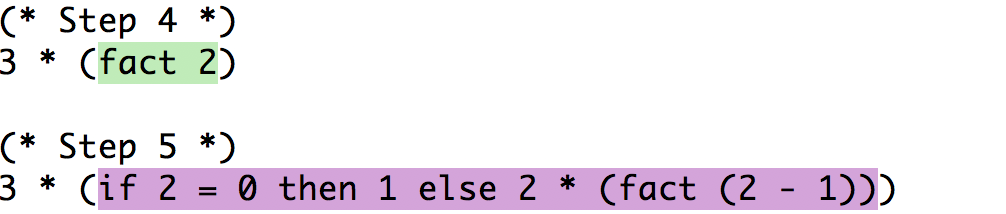
\includegraphics[height=2cm]{5/skip1.png}
  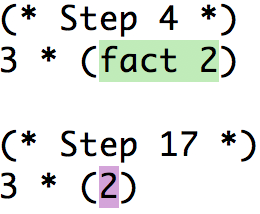
\includegraphics[height=2cm]{5/skip2.png}
  \caption{ステッパのスキップ機能}
  \label{figure:skip}
\end{figure}

また、著者らの incremental でないステッパ\cite{FSA18}は、プログラムの流れを理解する助けやステッパの利便性の向上のため、関数適用式が値に計算されるまでが1ステップであるかのように進める機能を有していた。図\ref{figure:skip} の左のように関数適用が簡約されるステップで Skip ボタンを押すと、図\ref{figure:skip} 右のように、下のプログラムが「関数適用式が値に簡約されたステップ」のプログラムに変わる。この状態で Next ボタンを押すとその続き、図\ref{figure:skip} の場合には \texttt{3 * 2 $\leadsto$ 6} のステップが表示される。これを本研究の incremental なステッパでも1ステップとして扱い、1度の実行で関数適用が値になるステップまでを計算し、その最後のステップを出力するように実装を進めている。そのためには、図\ref{figure:mode} の \texttt{mode} 型にスキップのためのコンストラクタを追加し、そのモードの場合には「実行している関数適用式が値になるステップまでは出力・終了を行わない」ようにするだけで良い。


\subsection{ツールの実装}

ここまで、ステッパ関数としてのステッパプログラムの実装を紹介した。
ユーザが incremental なステッパツールを使用するには、
ユーザの入力を受けてステッパプログラムを呼び出しステップを表示する外部のプログラムが必要になる。

DrRacket のステッパ\cite{clements01}や incremental でない OCaml ステッパでは、
外部のプログラムは「ステッパを起動して、出力を蓄えて、ユーザの操作に従って表示」をしていたが、
本研究のステッパでは、
「ユーザの操作に従ってステッパを呼び出して、出力されたものを装飾して表示」をする。
すると、外部のプログラムではステップ番号と前回の出力のみを保持することで実装が可能になる。


\section{予想される問題点とその経過}
本節では、incremental な OCaml ステッパを実際に利用するときに発生しうる問題点とその解決方法を挙げ、
大学の授業 ( \ref{section:experiment__course} 節で触れる) で利用してそれらが実際に問題になったかどうかを述べる。

\subsection{文字数の爆発}
\label{予想される問題点-文字数の爆発}

\subsubsection{問題点}

本章のステッパでは、
任意のステップの「処理用の出力」に入力プログラムからそこまでの簡約の過程が記されているため、
1ステップ進むごとに文字数が増加する。
具体的には、簡約基 \texttt{e1} が式 \texttt{e2} に簡約されるステップでは、
その時点のコンテキストを \texttt{E}、ステップ番号を \texttt{n} とすると、
簡約前のプログラムが \texttt{E[e1]}、
簡約後のプログラムが \texttt{E[e2[@stepper.reduct n;; e1]]} となる。
\texttt{E} の文字数は変わらないので、\texttt{e2[@stepper.reduct n;;}
と \texttt{]}の分の文字数が増加することになる。
これを続けていくと、1ステップあたり少なくとも22文字は増加することになり、
仮に百万ステップの簡約をするとプログラムは数千万文字になる。
すると、毎ステップの入出力や通信に時間がかかる可能性がある。

\subsubsection{解決方法}

解決策としては、古いステップの attribute は削除してしまうという方法が考えられる。
たくさんのステップを見てから最初の方のステップまで戻るユーザは少ないと仮定すれば、
ある程度前のステップについての attribute があったら、
関数 \texttt{memo} で出力するプログラムを再構成する際に消去すれば、
さほど実際の使用に影響なく出力する文字数を減らすことができる。

\subsubsection{使用した結果}

実際の incremental な OCaml ステッパ (\ref{実装-実際のステッパ} 節) では、
Emacs Lisp プログラムによってステッパ関数の実行や表示を制御する。
これを用いた授業では、文字数の多さが原因の不具合は報告されず、
1 ステップの入出力にかかる時間も利用に支障が出ない程度だった。

\subsection{実行時間}
\label{予想される問題点-実行時間}

\subsubsection{問題点}

ステップ数が膨大になると、後ろの方までステップ実行をするのは困難である。
incremental なステッパ関数での実行速度は通常の OCaml 処理系に決して及ばないので、
1ステップずつ進める場合でも、スキップ機能(\ref{実装-実際のステッパ}節)を使う場合でも、
実行を多く進めるには長い時間が掛かってしまう。

\subsubsection{解決方法}
少しでも急ぐ為には、一般的なデバッガのように、
ステップ実行したい式の付近にユーザがブレークポイントを設定して、
そこからステップ実行を始めるという方法が考えられる。
そのためには、ブレークポイントまでを部分的に native code にコンパイルして実行するなどの方法を取らざるを得ない。
しかしいずれにしても、
通常の OCaml コンパイラを用いても長時間かかるプログラムの実行を早く終わらせることは不可能である。

\subsubsection{使用した結果}

1 ステップずつ進める場合は、プログラムの実行を後ろの方まで進めることは困難であるが、
ステップごとの実行時間が問題になることはなかった。
スキップ機能を使用する場合は、やはり通常の OCaml で実行するよりも長い時間を要した。
具体的には、東京メトロ全線の駅についてダイクストラ法で最短路問題を解くプログラムの実行に、
通常の OCaml では 0.327 秒、incremental な OCaml ステッパではスキップ機能を使用して約 54 秒かかった。

\subsection{関数適用評価スキップ後の前ステップ出力}

\subsubsection{問題点}

関数適用をスキップ(\ref{実装-実際のステッパ}節)した後に前のステップに戻ろうとすると、
スキップで飛ばされたステップには戻ることができない。
たとえば図\ref{figure:skip}のように2の階乗の計算をスキップしたとすると、
図\ref{figure:skip}の右の状態から、incremental でないステッパでは
\begin{itemize}
\item スキップをする前の関数適用式が簡約されるステップ5(図\ref{figure:skip}左)
\item 関数適用式が最終的な値になるステップ17(
\texttt{3 * \colorbox{lightgreen}{(2 * 1)} $\leadsto$ 3 * \colorbox{purple}{2}})
\end{itemize}
のどちらにも戻ることができたが、incremental なステッパでは前者にしか戻ることができない。

その原因は、incremental でないステッパでは \ref{予想される問題点-実行時間}
節で述べたように文字列検索によってステップ表示を切り替えていたので任意のステップに移ることができたのに対して、
incremental なステッパではステッパ関数が関数適用式が値になるまでを1ステップとして出力し、
その間の簡約についての情報は出力しないからである。

\subsubsection{解決方法}

これを解決するには、
スキップする部分の計算をしている間の簡約についても attribute に情報を蓄え、
スキップ後のステップで全ての簡約の情報が入った長いプログラムを出力する必要がある。
しかしそのようにすると
\ref{予想される問題点-文字数の爆発} 節と
\ref{予想される問題点-実行時間} 節の問題がより深刻になる可能性がある。

\subsubsection{使用した結果}

ステッパを利用した学生に答えてもらったアンケートに
「ステッパの不便なところ、欲しい機能などがあれば教えてください。」
という質問を含めたが、この点に関する要望は出なかった。


\section{まとめと今後の課題}

本研究では、OCaml のプログラムの簡約による書き換えを1ステップずつ見せるプログラムであるステッパを、1度の実行で1つの簡約のみを行うように変更し、ステッパの起動時間を短縮した。またそのためにあるステップのプログラムからそれ以前のステップのプログラムを計算できるようにする必要が生まれたので、それまでの簡約の内容を全て記録したプログラムを出力することで入力プログラムの情報が失われないように変更した。

今後は、一部の副作用を伴うプログラムに対応することを目指す。incremental でない OCaml ステッパ\cite{FSA18} はこれらに対応しているが、incremental になり、ストアや標準出力された文字列の情報をステッパのプロセスが保持できなくなったことで、ストアの情報もステッパの出力に含める必要が生じた。これは恐らく、プログラムの attribute (\ref{OCamlのattribute-プログラムのattribute}節)を利用することで解決できるであろう。
